\chapter{Absolute intensities, moments and volume fractions}
\label{ch:absint}

\section{Fitting absolute intensities}

Absolute intensities in the simulation can be obtained by using
proper units for the scattering vector $\mathbf{Q}$, the size
dimensions of the scatterer, the scattering length densities etc. In
the following a few example are discussed for absolute calibrated
data sets. One question which is asked quite frequently is "What is
the meaning of $N$ in the size distribution and what are its units?".
The answer is normally "That depends on the units of your data you
are fitting and the units of your scattering length densities". In
the following a few explanations will be given to clarify this in
some more detail.

Let us consider first the scattering intensity of a single sphere.
The form factor of a sphere is given by eq.\ \ref{eq:I_sphere} as
\begin{align}
I_\text{Sphere}(Q,R,\Delta\eta) =  \left[\frac{4}{3}\pi R^3 \Delta\eta \, 3
\frac{\sin QR - QR \cos QR}{(QR)^3} \right]^2
\end{align}
The radius $R$ and the scattering vector $Q$ have reciprocal units,
i.e. if $Q$ is given in $1/\mathrm{nm}$ the radius $R$ has a unit of
nm. The other variable in the form factor is the scattering length
density contrast $\Delta\eta$ between sphere and surrounding matrix
or solvent. The unit of the scattering length density is
length/volume and has therefore a unit $1/\mathrm{cm}^2$ or some
other sites are using units of $1/\mathrm{{\AA}}^2$. The difference is only a
constant factor of
\begin{align}
\Delta\eta \frac{1}{\textrm{cm}}=
10^{16} \Delta\eta\, \frac{1}{\textrm{\AA}}.
\end{align}
The overall unit of the scattering intensity (differential cross-section)
of a single sphere is therefore
\begin{align}
\left[ I_\text{Sphere}(Q,R,\Delta\eta) \right] =
\left[R\right]^6 \left[\Delta\eta\right]^2 =
\frac{\textrm{nm}^6}{\textrm{cm}^4} =
10^{-42} \textrm{cm}^2
\end{align}
for the case that $[R]=\textrm{nm}$ and
$[\Delta\eta]=\textrm{cm}^{-2}$. The unit for the scattering
cross-section of a single sphere with $[R]=\textrm{\AA}$ and
$[\Delta\eta]=\textrm{\AA}^{-2}$ is than
\begin{align}
\left[ I_\text{Sphere}(Q,R,\Delta\eta) \right] =
\left[R\right]^6 \left[\Delta\eta\right]^2 =
\frac{\textrm{\AA}^6}{\textrm{\AA}^4} = \textrm{\AA}^2 =
10^{-16} \textrm{cm}^2,
\end{align}
respectively. The scattering cross-section of a single scatterer is calculated by
\SASfit if one chooses in the tab for distribution functions the probability
functions \texttt{Monodisperse}.

Differential cross-section have a unit of an area
\begin{align}
\left[\frac{d\Sigma}{d\Omega}(Q)\right] = \textrm{cm}^2.
\end{align}
Many instruments deliver with their data reduction software a
cross-section normalized by the sample volume so that the unit is in
reciprocal length:
\begin{align}
\left[\frac{d\sigma}{d\Omega}(Q)\right]
= \frac{1}{\left[V\right]}\left[\frac{d\Sigma}{d\Omega}(Q)\right]
= \frac{1}{\textrm{cm}}
.
\end{align}

For fitting a form factor to experimental data one needs next to the size parameter also a
scaling parameter. For the simplest case this is done by choosing as a distribution function
\texttt{Delta}. \texttt{Delta} simply multiplies a constant value $N$ to the form factor.
The meaning and the unit of $N$ now depends on the unit of the cross-section, wether it is
normalized or not normalized on the sample volume. \SASfit calculates in the case of
a form factor of \texttt{Sphere} with \texttt{Delta} as a distribution function
\begin{align}
I_\text{\SASfit} = N \times I_\text{Sphere}(Q,R,\Delta\eta).
\end{align}
Fitting $N$ to a data set, which is given in units of 1/cm and where $[Q]=\textrm{nm}^{-1}$, $[R]=\textrm{nm}$
and $[\Delta\eta]=\textrm{cm}^{-2}$ would mean that $N$ has the unit
\begin{align}
\left[ N \right] = \frac{\left[\frac{d\sigma}{d\Omega}(Q)\right]}{\left[I_\text{Sphere}(Q,R,\Delta\eta)(Q)\right]}
= \frac{\frac{1}{\textrm{cm}}}{10^{-42}\textrm{cm}^2} = 10^{42} \textrm{cm}^{-3}.
\end{align}
One therefore needs to multiply the value $N$ obtained by \SASfit
with $10^{42}$ to get the number density of scatterers in units of cm$^{-3}$.

Let us now consider the simplest case of spheres with a size distribution and no structure factor,
which are fitted to experimental data. All the size distribution have a scaling parameter $N$.
The units of the parameter $N$ in the size distribution is the same than for \texttt{Delta}.
The size distribution $n(x)$ are implemented as distribution function $n(x) = N p(x)$ with $p(x)$
being a probability function. In case of polydisperse spheres \SASfit calculates the integral
\begin{align}
I_\text{\SASfit} (Q)
&= \int_0^\infty n(R) \, I_\text{Sphere}(Q,R,\Delta\eta) \, dR \\
&= N \int_0^\infty p(R) \, I_\text{Sphere}(Q,R,\Delta\eta) \, dR
\end{align}
The probability function $p(x)$ is normalized to
\begin{align}
\int_0^\infty p(x) \, dx = 1,
\end{align}
so that the parameter $N$ has like for the
\texttt{Delta}-distribution the unit $\left[ N \right]= 10^{42}
\textrm{cm}^{-3}$ if the data set is given in units of 1/cm and
$[Q]=\textrm{nm}^{-1}$, $[R]=\textrm{nm}$ and
$[\Delta\eta]=\textrm{cm}^{-2}$.

Most of the form factor are implemented in a way that they return
the scattering cross-section of a single object like the example of
a sphere above, but a few are not, like for example the standard
form of a gaussian chain \texttt{Gauss}. In this particular case two
other versions \texttt{Gauss2} and \texttt{Gauss3} with different
parameterizations of the forward scattering of a single gaussian
chain are available. However, there are some form factors, which
have been implemented according to the literature but which are
normalized differently. This has to be checked before the parameter
$N$ in the size distribution is interpreted in terms of number
density of scatterers.

\section{Contrast - Concentration - Forward Scattering - Particle Volume - Absolute Scale}
\label{sec:contrast-concentration-I(0)}

A frequently asked question is if the scattering intensity is consistent
with the concentration of material in the sample. Especially people working with micellar solution,
star polymers, but also proteins, etc. want to cross-check the absolute intensity with the known concentration.
In the dilute case the differential cross-section is simply $N$ times the cross-section of an individual scatterer
\begin{align}
\frac{d\sigma}{d\Omega}(Q) &= \frac{N}{V_\text{tot}} P(Q)
\label{eq:xsabsolut1}
\end{align}
$N$ is number of particles/molecules/proteins in the illuminated volume,
$V_\text{tot}$ the illuminated sample volume,
$n=N/V_\text{tot}$ the particle number density,
and $P(Q)$ the scattering cross-section of a single particle.
$P(Q)$ has the dimension cm$^{2}$, $N/V_\text{tot}$ the dimension cm$^{-3}$,
and $\frac{d\sigma}{d\Omega}(Q)$ the dimension cm$^{-1}$. Eq.\ \ref{eq:xsabsolut1}
can also be expressed in terms of concentration $c$ in units of $\mathrm{g}/\mathrm{cm}^2$
\begin{align}
c &= n\; m_\text{mol} = n\; M_r u = n\frac{M_rM_u}{N_A} =
\frac{N}{V_\text{tot}}\frac{M_r M_u}{N_A}
\end{align}
so that
\begin{align}
\frac{d\sigma}{d\Omega}(Q) &= c\frac{N_A}{M_r M_u} P(Q)
\label{eq:xsabsolut1}
\end{align}
$M_r$ is the relative molar mass of the particle
\footnote{
Definition of relative atomic mass and relative molecular mass can be found on the url-address
http://physics.nist.gov/Pubs/SP811/sec08.html
\begin{description}
\item[Relative atomic mass (formerly atomic weight)] ratio of the average mass per atom of an element to 1/12 of the mass of the atom of the nuclide $^{12}$C.
\item[Relative molecular mass (formerly molecular weight)] ratio of the average mass per molecule or specified entity of a substance to 1/12 of the mass of an atom of the nuclide $^{12}$C.
\end{description}
}
 (Molecular weight (M.W.) and formula weight (F.W.) are older terms) which is a
dimensionless quantity (i.e., a pure number, without units). To get
units in g/mol the relative molar mass needs to be multiplied by the
molar mass constant $M_u$.
The value of the molar mass constant $M_u$ is defined to be 1 g/mol in SI
units. The molar mass constant is important in writing
dimensionally correct equations. It is common to see phrases such
as "\emph{The molar mass of an element is the atomic weight in
grams per mole.}" However molecular or atomic weight are
dimensionless quantities, and cannot take the units of grams per
mole. Formally, the operation is the multiplication by a constant
which has the value 1 g/mol, that is the molar mass
constant\footnote{Definition of unified atomic mass unit: $1 \mathrm{u} = m_{\mathrm{u}} = m\left({}^{12}\mathrm{C}\right) / 12 = 1M_u/N_A=1\left(\mathrm{g}/\mathrm{mol}\right) / \left(6.02214129\times 10^{23} \mathrm{mol}^{-1}\right)=1.660538921\times 10^-{24}\mathrm{g}$}.
The molecule mass $m_\text{m}$ in units of g is $m_\text{m}=M_r M_u/N_A$.

Now we need to look on the forward scattering $P(Q\mbox{$=$}0)$ of a single particle/protein/polymer chain.
For a simple particle like a sphere, the forward scattering is given by
\begin{align}
P(Q\mbox{$=$}0) &= \left(\eta_\mathrm{sol}-\eta_\mathrm{sp}\right)^2 V_\mathrm{sp}^2
\end{align}
where $\left(\eta_\mathrm{sol}-\eta_\mathrm{sp}\right)$ is the scattering contrast between
spherical particle and solvent and $V_\mathrm{sp}$ the volume of a single sphere. In case of a spherical
particle the boundary between particle and solvent is well defined and therefore also the volume of the particle
as it has a sharp interface. The scattering contrast of a spherical particle
can also be written in terms of the overall scattering length of the sphere $b_\mathrm{sp}$,
i.e. the sum of the scattering length of all atoms forming the sphere,
the volume of the sphere and the scattering length density of the solvent.
The volume of the sphere can be calculated from its mass $m_\mathrm{sp}$ or
relative molar mass $M_{r,\mathrm{sp}}$
and its density $\rho_\mathrm{sp}$.
\begin{align}
\left(\eta_\mathrm{sol}-\eta_\mathrm{sp}\right)
&= \left(\eta_\mathrm{sol}-\frac{b_\mathrm{sp}}{V_\mathrm{sp}}\right)
 = \left(\eta_\mathrm{sol}-\frac{b_\mathrm{sp} \rho_\mathrm{sp}}{m_\mathrm{sp}}\right)
 = \left(\eta_\mathrm{sol}-\frac{b_\mathrm{sp} \rho_\mathrm{sp} N_A}{M_{r,\mathrm{sp}}M_u}\right)
\end{align}
But what about the forward scattering of a gaussian polymer coil? A polymer does not has a sharp boundary
to the solvent. Polymer and solvent can penetrate each other. To determine the polymer volume one would need
a detailed model for the polymer molecule and its interaction with solvent molecules.
As a first approximation the volume of a polymer molecule can be obtained by
$V_\mathrm{polym}=\frac{\rho_\mathrm{polym}}{m_\mathrm{polym}}$.
For a polymer coil with a relative molar mass $M_{r,\mathrm{polym}}$ the forward scattering in a solvent is given by
\begin{align}
P(Q\mbox{$=$}0)
&= \left(\frac{M_{r,\mathrm{polym}}M_u}{\rho_\mathrm{polym} N_A}\right)^2
\left(\eta_\mathrm{sol}-\frac{b_\mathrm{polym} \rho_\mathrm{polym} N_A}{M_{r,\mathrm{polym}}M_u}\right)^2
\end{align}
The  volume of a polymer molecule
\[
V_\mathrm{polym} = \frac{M_{r,\mathrm{polym}}M_u}{\rho_\mathrm{polym} N_A}
\]
is the volume occupied by single polymer chain in the solvent or in other word the amount
of solvent volume displaced by one polymer chain.
For the forward scattering it does not matter, if the coil is collapsed or swollen.
As long as the scattering length density of the solvent inside the swollen polymer coil is the
same than in the bulk and the molecular volume of the polymer chain does not change with
the solvent quality the forward scattering does not depend on the conformation of the polymer.
Sometimes the relative molar mass of a polymer is given in degree of polymerization $p$
and relative molar mass of the monomer $M_{r,\mathrm{m}}$.
In this case and assuming that the mass densities of polymer and monomer are the same
the forward scattering is given by
\begin{align}
P(Q\mbox{$=$}0)
&= \left(\frac{p\; M_{r,\mathrm{m}}M_u}{\rho_\mathrm{m} N_A}\right)^2 \left(\eta_\mathrm{sol}-\frac{b_\mathrm{m} \rho_\mathrm{m} N_A}{M_{r,\mathrm{m}}M_u}\right)^2 \nonumber \\
&= \left(\frac{p\; M_{r,\mathrm{m}}M_u}{\rho_\mathrm{m} N_A}\right)^2 \left(\eta_\mathrm{sol}-\frac{b_\mathrm{m} \rho_\mathrm{m} N_A}{M_{r,\mathrm{m}}M_u}\right)^2
\end{align}
Let us now come back to the measured differential cross-section $\frac{d\sigma}{d\Omega}(Q)$. For
$Q=0$ we get
\begin{align}
\frac{d\sigma}{d\Omega}(Q\mbox{$=$}0) &= \frac{N}{V_\text{tot}} P(Q\mbox{$=$}0) = c\frac{N_A}{M_{r,\mathrm{Gauss}} M_u} P(Q\mbox{$=$}0) \\
&= c\; \frac{N_A}{p\; M_{r,\mathrm{m}} M_u} \left(\frac{p\; M_{r,\mathrm{m}}M_u}{\rho_\mathrm{m} N_A}\right)^2 \left(\eta_\mathrm{sol}-\frac{b_\mathrm{m} \rho_\mathrm{m} N_A}{M_{r,\mathrm{m}}M_u}\right)^2 \\
&= c\; \frac{p\; M_{r,\mathrm{m}} M_u}{N_A \rho_\mathrm{m}^2} \left(\eta_\mathrm{sol}-\frac{b_\mathrm{m} \rho_\mathrm{m} N_A}{M_{r,\mathrm{m}}M_u}\right)^2
\end{align}
The last equation says, that the forward scattering of a solution of dilute non-interacting polymer molecules
consisting of $p$ monomer units depends linearly on the number of monomer units $p$ in the polymer.
Even though the scattering of a single polymer molecule depends quadratically on on the number of monomer units.
The reason is simply that the larger the degree of polymerization the lower the number density of molecules in the solution
as we assume a constant concentration, i.e. $c\propto pn$ and therefore $\frac{d\sigma}{d\Omega}(Q\mbox{$=$}0) \propto p^2n$.

\section{Moments of scattering curves and size distribution}
\label{sec:SASmoments}

The relevance of moments both for scattering curves as well as size
distributions has been discussed in several publications
\cite{Damaschun1969,Sjoberg1974,Damaschun1971,Walter1985,Moller1995,book:Guinier:Fournet}.

Moments $ \langle x^m\rangle$ of any order $m$ of a function $f(x)$
are defined by integrating $f(x)$  with a suitable power of $x$ over
its domain $[a,b]$
\begin{align}
 \langle x^m\rangle = \displaystyle  \int_a^b f(x) x^m dx
\end{align}

The different moments of the scattering curve together with the
forward scattering $I(0)$ and the Porod constant can be used to
calculate easily several structural parameters of the scatterers.
\begin{subequations}
\begin{align}
\tilde{Q}_\text{inv} &= \int_0^\infty Q^2I(Q) \mathrm{d}Q \mbox{ (scattering invariant)} \\
\frac{S}{V} &= \frac{\pi}{\tilde{Q}_\text{inv}} \;\; {\DS\lim_{Q \to \infty}\left\{Q^4I(Q)\right\}} \mbox{ (specific surface)} \\
\langle R_G \rangle^2 &= 3\left(-\DS\lim_{Q \to 0}\left\{\frac{\mathrm{d}[\ln I(Q)]}{\mathrm{d}(Q^2)}\right\}\right) \mbox{ (squared Guinier radius)} \\
l_i=\langle d \rangle &= \frac{4}{\pi}\frac{\int_0^\infty Q^2I(Q) \mathrm{d}Q}{\DS\lim_{Q \to \infty}\left\{Q^4I(Q)\right\}} \mbox{ (average intersection length)} \\
l_c=\langle l \rangle &= \frac{\pi}{\tilde{Q}_\text{inv}} \int_0^\infty QI(Q) \mathrm{d}Q \mbox{ (correlation length)} \\
A_c=\langle A \rangle &= \frac{2\pi}{\tilde{Q}_\text{inv}}\int_0^\infty I(Q) \mathrm{d}Q \mbox{ (correlation surface)} \\
V_P=\langle V \rangle &= \frac{2\pi^2}{\tilde{Q}_\text{inv}} I(0)
\mbox{ (correlation volume, Porod volume)}
\end{align}
\end{subequations}
These structural parameters are calculated by \SASfit via the menu
\texttt{[Calc|integral parameters...]}.


\begin{figure}[htb]
\begin{center}
\subfigure[GUI for defining fit ranges for Porod and Guinier
approximations]{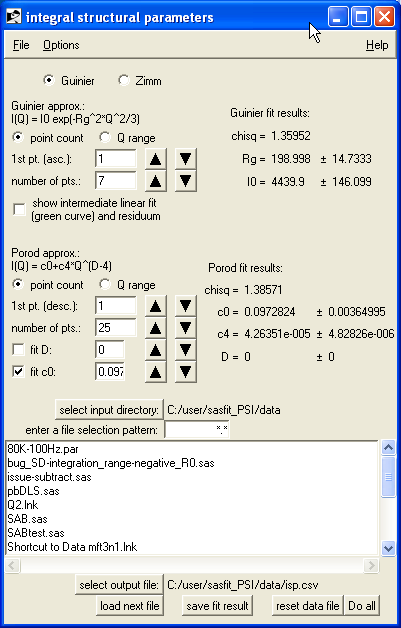
\includegraphics[width=0.296\textwidth,height=0.464\textwidth]{QTintegralparameterGUI.png}}
\hfill \subfigure[Tabbed menu displaying the integral structural
parameters calculated via the different moments of the scattering
curve the Porod and Guinier extrapolations to $Q\rightarrow 0$ and
$Q\rightarrow\infty$.
]{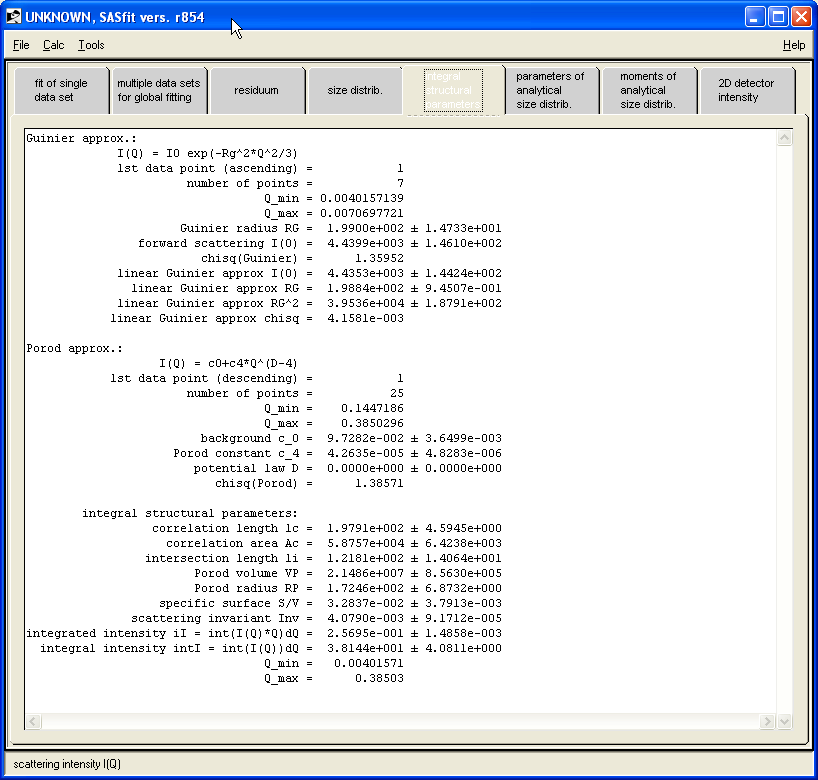
\includegraphics[width=0.604\textwidth,height=0.576\textwidth]{QTintegralparameterTab.png}}
\end{center}
\caption{Menu and tabbed window for integral structural parameters.
\SASfit also supports analysis of series of data, whereby the
structural parameters are stored in CSV format readable by many
software packages in a separate file for further analysis.}
\label{fig:QTintegralstructuralparameters}
\end{figure}


On the other side the structural parameters from above can depend on
specific moments of the size distribution in the case the scattering
objects are spheres.
 The $m$-th moment $\langle x^m\rangle$ of a size
distribution $n(R)$ is given by
\begin{align}
 \langle R^m\rangle = \frac{\displaystyle  \int_0^\infty n(R) R^m dR }{
\displaystyle \int_0^\infty n(R) dR}
\end{align}
From these moments the following integral structural parameters in
case of polydisperse spheres can be calculated and are listed
together with a hypothetical radius of monodisperse spheres having
the same structural parameter.

~\\
\begin{description}
\item[intersection length $l_i$]~\\
$\displaystyle l_i = \frac{\langle R^3\rangle}{\langle R^2\rangle}
$ and  $\displaystyle R_{l_i} = \frac{3}{4} l_i $

\item[correlation length $l_c$]~\\
$\displaystyle l_c = \frac{\langle R^4\rangle}{\langle R^3\rangle}
$ and  $\displaystyle R_{l_c} = \frac{2}{3} l_c $

\item[Guinier radius $R_G$]~\\
$\displaystyle R_G = \sqrt{\frac{\langle R^8\rangle}{\langle
R^6\rangle}} $ and  $\displaystyle R_{R_G} = \sqrt{\frac{5}{3}}
R_G $

\item[correlation cross section $A_c$]~\\
$\displaystyle A_c = \frac{4\pi}{5}\frac{\langle
R^5\rangle}{\langle R^3\rangle} $ and  $\displaystyle R_{A_c} =
\sqrt{\frac{5}{4\pi} A_c} $

\item[Porod Radius $R_{V_P}$]~\\
$\displaystyle V_P = \frac{4\pi}{3}\frac{\langle
R^6\rangle}{\langle R^3\rangle} $ and  $\displaystyle R_{V_P} =
\sqrtthree{\frac{3}{4\pi} V_P} $
\end{description}


\begin{figure}[htb]
\begin{center}
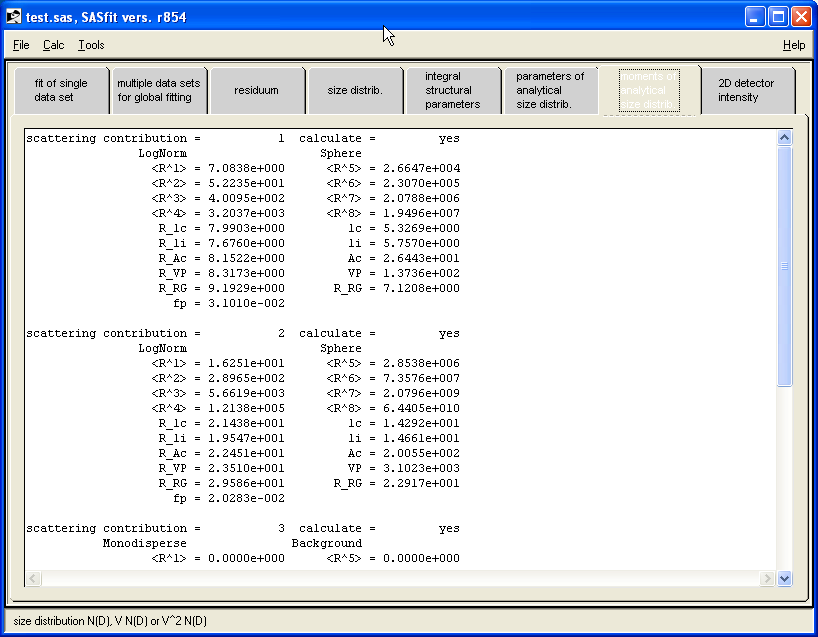
\includegraphics[width=0.818\textwidth,height=0.637\textwidth]{QTmoments.png}
\end{center}
\caption{Menu displaying the different moments of a size
distribution. At the moment these values are only calculated for
single data sets but not yet for multiple data sets}
\label{fig:QTmoments}
\end{figure}

Fig.\ \ref{fig:QTmoments} shows the \SASfit menue displaying these
values for each scattering contribution having a size distribution
and also for the sum of all scattering contributions. Next to the
integral structural parameters also the different moments of the
size distribution up the the $8^\textrm{th}$ moment are supplied.

\section{Volume fractions}
\label{sec:volumefraction}

Having measured SAS-data versus $[Q]=nm^{-1}$ in absolute scale
(1/cm) and knowing the scattering contrast also in absolute scale
(1/cm$^2$) one can get the number density of particles. However, in
general the volume fraction is known by other means but not the
number density. The volume fraction can be calculated from the size
distribution for some simple geometric shapes of the particles.


Let us first consider the case of simple spheres (\texttt{Sphere})
with a size distribution over there radii. The size distribution can
be interpreted as a number density distribution function. The volume
fraction $f_p$ of the spheres can be easily calculated by
\begin{align}
f_p = \int_0^\infty n(R) \frac{4}{3}\pi R^3 \, dR
    = \int_0^\infty N p(R) \frac{4}{3}\pi R^3 \, dR
    = N \frac{4}{3}\pi \langle R^3 \rangle
\label{eq:fpMomentSphere}
\end{align}
where $\langle R^3 \rangle$ is the third moment of the size
distribution. The different moments of a size distribution can be
calculated analytically for some special cases like the lognormal
distribution. However, \SASfit calculates the moments and displays
them on the menu \verb"[calc|single data single]". Up to the
8$^\textrm{th}$-moment of a distribution function is displayed in
the menu tab \texttt{moments of analytical size distrib.} like in
Fig.\ \ref{fig:QTmoments} together with some other parameters
defined in section \ref{sec:SASmoments}. To compute the volume
fraction $f_p$, which is a dimensionless parameter, one has to use
the proper units for $N$ and $\langle R^3 \rangle$. $\langle R^3
\rangle$ has here units of $\left[\langle R^3
\rangle\right]=\textrm{nm}^3=10^{-21}\textrm{cm}^3$ and $N$ is in
units of $\left[N\right]=10^{42}\textrm{cm}^{-3}$. The volume
fraction $f_p$ can as an example be computed for $N=8.55241\times
10^{-28}$ and $\langle R^3 \rangle=5.6619\times 10^{3}$ as
\begin{align}
f_p=10^{42}\times 8.55241\times 10^{-28} \, \frac{4}{3}\pi \, 5.6619\times 10^{3} \, 10^{-21}=0.020283.
\label{eq:fpMoments_eg}
\end{align}
The numbers for $N$ and $\langle R^3 \rangle$ can be directly taken from the \SASfit gui.

Let us now consider the case of cylinders with a circular
cross-section with radius $R$ and length $L$. We will have a look on
the two cases of having either a distribution in the radius $R$ or a
distribution in the length $L$. The volume of a cylinder
$V_\textrm{cyl}$ is given by
\begin{align}
V_\textrm{cyl}(R,L) = \pi R^2 L
\end{align}
To calculate the volume fraction from the size distribution we need
to integrate over the particle volume. The integration is done
either over the radius $dR$
\begin{align}
f_p = \int_0^\infty n(R) V_\textrm{cyl}(R,L) \, dR
    = \int_0^\infty N p(R) \pi R^2 L \, dR
    = N L \pi \langle R^2 \rangle
\label{eq:fpMomentsCylR}
\end{align}
or over the cylinder length $dL$
\begin{align}
f_p = \int_0^\infty n(L) V_\textrm{cyl}(R,L) \, dL
    = \int_0^\infty N p(L) \pi R^2 L \, dL
    = N R^2 \pi \langle L \rangle
\label{eq:fpMomentsCylR}
\end{align}
depending if we have a distribution over the radius $R$ or the
length $L$. In both cases the volume fraction can be expressed in
terms of moments of the size distribution supplied by {\tt SASfit}.
In the first case it can be expresses by the second moment $\langle
R^2 \rangle$ of the cylinder radius and in the second case by the
first moment $\langle L \rangle$ of the cylinder length, i.e. the
mean cylinder length. The required moments are displayed in \SASfit
in the menu shown in Fig.\ \ref{fig:QTmoments}. Also here one has to
take care using proper units, but this is done equivalently to the
first example of a sphere in eq.\ \ref{eq:fpMoments_eg}.

The three examples above show that the volume fraction $f_p$ of
scatterers can be calculated in many cases via the moments of the
size distribution and for simple cases all necessary parameters are
supplied in the \SASfit menu interface. The volume fraction
\texttt{fp} in Fig.\ \ref{fig:QTmoments} is numerically calculated
from the size distribution. For some specific other form factor and
the special case of a \texttt{LogNorm} distribution a plugin size
distribution named \texttt{LogNorm\_fp} described in section
\ref{sec:sd_lognorm_fp} has been implemented. Calculating volume
fractions for any size distribution and for any form factor is not
easy to implement. It would require quite some knowledge about the
form factor and how exactly the volume fraction is defined. The
plugin \texttt{LogNorm\_fp} distinguish between volume fraction of a
core only, a volume fraction of a core together with a shell and a
volume fraction of a shell only. For the general case one also needs
to know which size parameter of the form factor has a distribution.
This already shows that the user has to supply additional
information. For the calculation a volume function has to be
associated to each form factor. If this is not the case the \SASfit
routine returns 0. For those function a volume function is
associated to the form factor \SASfit calculates numerically the
volume fraction for any size distribution by integration. The plugin
function \texttt{LogNorm\_fp} on the other side has a lognormal
distribution implemented and the information about the form factor
and the size parameter of the form factor having a distribution has
to be given by the user via an input value called \texttt{shape}.
Only a very limited number of form factor can be selected by this
parameter. For other form factors the plugin needs to be extended or
an routine calculating the volume for the specific form factor needs
to be implemented.
